
% This LaTeX was auto-generated from MATLAB code.
% To make changes, update the MATLAB code and republish this document.

\documentclass{article}
\usepackage{graphicx}
\usepackage{color}

\sloppy
\definecolor{lightgray}{gray}{0.5}
\setlength{\parindent}{0pt}

\begin{document}

    
    

\section*{17. Orthogonal polynomials}

\begin{verbatim}
ATAPformats
\end{verbatim}
\begin{par}
 This book gives special attention to Chebyshev polynomials, since
they are so useful in applications and the analogue on $[-1,1]$
of trigonometric polynomials on $[-\pi,\pi]$.
However, Chebyshev polynomials are
just one example of a family of orthogonal polynomials defined on the
interval $[-1,1]$, and in this chapter we note some of the other
possibilities, especially Legendre polynomials, which are the starting
point for Gauss quadrature (Chapter 19).  The study of orthogonal
polynomials was initiated by Jacobi [1826] and already well developed by
the end of the 19th century thanks to work by mathematicians including
Chebyshev, Christoffel, Darboux, and Stieltjes. Landmark books on the subject
include Szeg\H o [1939] and Gautschi [2004]. 
\end{par} \vspace{1em}
\begin{par}

Let $w\in C(-1,1)$ be a {\em weight function} with $w(x) > 0$ for all
$x\in (-1,1)$ and $\int_{-1}^1 w(x) \kern .4pt dx <\infty$; we allow
$w(x)$ to approach $0$ or $\infty$ as $x \to\pm 1$. The function $w$
defines an {\em inner product} for functions defined on $[-1,1]$:
$$ (f,g) = \int_{-1}^1 w(x) \kern .4pt \overline{f(x)}
\kern .4pt g(x) \kern .4pt dx . \eqno (17.1) $$
(The bar over $f(x)$ indicates the complex conjugate, and can be ignored
when working with real functions.)
A family of {\em orthogonal polynomials} associated with $w$ is a family
$$ p_0  , p_1, p_2, \dots $$
where $p_n$ has degree exactly $n$ for each $n$ and the
polynomials satisfy the orthogonality condition
$$ (\kern .7pt p_j,p_k) = 0, \quad k \ne j. \eqno (17.2) $$
Notice that this condition implies that each $p_n$ is orthogonal to all
polynomials of degree $k<n$. The condition (17.2) determines the family
uniquely except that each $p_n$ can be multiplied by a constant factor.
One common normalization is to require that each $p_n$ be monic, in which
case we have a family of {\em monic orthogonal polynomials}. Another
common normalization is $p_0>0$ together with the condition
$$ (\kern .7pt p_j , p_k) = \delta_{jk}
= \cases{1 & $k=j$,\cr 0 & $ k\ne j$,} \eqno (17.3) $$
in which case we have {\em orthonormal polynomials}. A third choice, the
standard one for Chebyshev and Legendre polynomials, is to require
$p_n(1) = 1$ for each $n$.

\end{par} \vspace{1em}
\begin{par}
As we have seen in Chapter 3, the Chebyshev polynomials $\{T_k\}$ are orthogonal with respect to the weight function $$ w(x) = {2\over \pi\sqrt{1-x^2}\kern .7pt } \eqno (17.4) $$ (Exercise 3.7).  If fact, if $T_0$ is replaced by $T_0/\sqrt 2$, they are orthonormal. The first three Chebyshev polynomials are $$ T_0(x) = 1, \quad T_1(x) = x, \quad T_2(x) = 2x^2 - 1, $$ as we can confirm with the \texttt{chebpoly} command:
\end{par} \vspace{1em}
\begin{par}
 \vskip -2em 
\end{par} \vspace{1em}
\begin{verbatim}
for j = 0:5, disp(fliplr(poly(chebpoly(j)))), end
\end{verbatim}

        \color{lightgray} \begin{verbatim}     1
     0     1
    -1     0     2
     0    -3     0     4
     1     0    -8     0     8
     0     5     0   -20     0    16
\end{verbatim} \color{black}
    \begin{par}
The Chebyshev weight function has an inverse-square root singularity at each end of $[-1,1]$.  Allowing arbitrary power singularities at each end gives the \textit{Jacobi weight function} $w(x) = (1-x)^\alpha (1+x)^\beta$, where $\alpha,\beta > -1$ are parameters.  The associated orthogonal polynomials are known as \textit{Jacobi polynomials} and written $\{P_n^{(\alpha,\beta)}\}$. In the special case $\alpha=\beta$ we get the \textit{Gegenbauer} or \textit{ultraspherical polynomials.}
\end{par} \vspace{1em}
\begin{par}

The most special case of all is $\alpha=\beta=0$, leading to
{\em Legendre polynomials}, with the simplest of all weight functions,
a constant:
$$ w(x) = 1. $$
If we normalize according to (17.3), the first three Legendre polynomials
are
$$ p_0(x) = \sqrt{1/2}, \quad p_1(x) = \sqrt{3/2}\kern 1.2pt  x, \quad
p_2(x) = \sqrt{45/8}\kern 1.2pt x^2 - \sqrt{5/8}, $$
as we can confirm by using the flag \verb|'norm'| with the {\tt legpoly} command:

\end{par} \vspace{1em}
\begin{par}
 \vskip -2em 
\end{par} \vspace{1em}
\begin{verbatim}
format short
for j = 0:5, c = fliplr(poly(legpoly(j,'norm'))); disp(c), end
\end{verbatim}

        \color{lightgray} \begin{verbatim}    0.7071
   -0.0000    1.2247
   -0.7906   -0.0000    2.3717
    0.0000   -2.8062   -0.0000    4.6771
    0.7955   -0.0000   -7.9550    0.0000    9.2808
    0.0000    4.3973   -0.0000  -20.5206    0.0000   18.4685
\end{verbatim} \color{black}
    \begin{par}
However, as mentioned above, it is more common to normalize Legendre polynomials by the condition $p_j(1) = 1$.  Switching to an upper-case $P$ to follow the usual notation, the first three Legendre polynomials are $$ P_0(x) = 1, \quad P_1(x) = x, \quad P_2(x) = \textstyle{3\over 2}x^2 - \textstyle{1\over 2}. $$ These are the polynomials returned by \texttt{legpoly} by default:
\end{par} \vspace{1em}
\begin{par}
 \vskip -1.5em 
\end{par} \vspace{1em}
\begin{verbatim}
for j = 0:5, c = fliplr(poly(legpoly(j))); disp(c), end
\end{verbatim}

        \color{lightgray} \begin{verbatim}    1.0000
   -0.0000    1.0000
   -0.5000   -0.0000    1.5000
    0.0000   -1.5000   -0.0000    2.5000
    0.3750   -0.0000   -3.7500    0.0000    4.3750
    0.0000    1.8750   -0.0000   -8.7500    0.0000    7.8750
\end{verbatim} \color{black}
    \begin{par}
The rest of this chapter is devoted to comparing Legendre and Chebyshev polynomials. The comparison, and the consideration of orthogonal polynomials in general, will continue into the next two chapters on rootfinding (Chapter 18) and quadrature (Chapter 19). For example, Theorem 19.6 presents a fast method for calculating the barycentric weights for \textit{Legendre points,} the zeros of Legendre polynomials.  On the whole, different families of orthogonal polynomials have similar approximation properties, but Chebyshev points have the particular advantage that one can convert back and forth between interpolant and expansion by the FFT.
\end{par} \vspace{1em}
\begin{par}
We begin with a visual comparison of the Chebyshev and Legendre polynomials of degrees 1--6 for $x\in[-1,1]$.  The shapes are similar, with the degree $n$ polynomial always having $n$ roots in the interval (Exercise 17.4).
\end{par} \vspace{1em}
\begin{par}
 \vskip -2em 
\end{par} \vspace{1em}
\begin{verbatim}
disp('              Chebyshev                     Legendre')
ax = [-1 1 -1 1]; T = []; P = [];
for n = 1:6
    T{n} = chebpoly(n);
    subplot(3,2,1), plot(T{n}), axis(ax), grid on
    P{n} = legpoly(n);
    subplot(3,2,2), plot(P{n},'m'), axis(ax), grid on, snapnow
end
\end{verbatim}

        \color{lightgray} \begin{verbatim}              Chebyshev                     Legendre
\end{verbatim} \color{black}
    
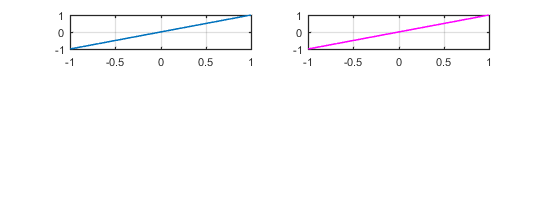
\includegraphics [width=4in]{chap17_01.png}

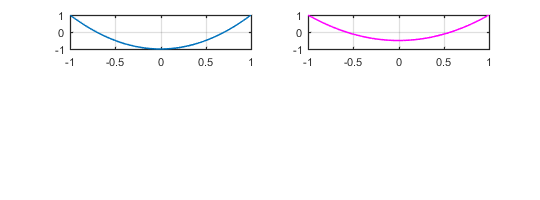
\includegraphics [width=4in]{chap17_02.png}

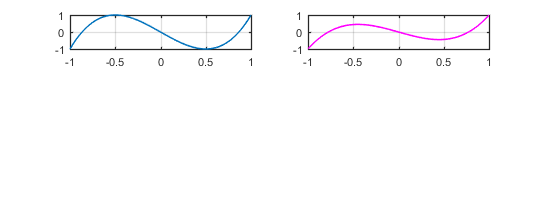
\includegraphics [width=4in]{chap17_03.png}

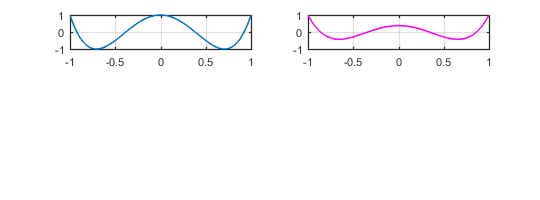
\includegraphics [width=4in]{chap17_04.png}

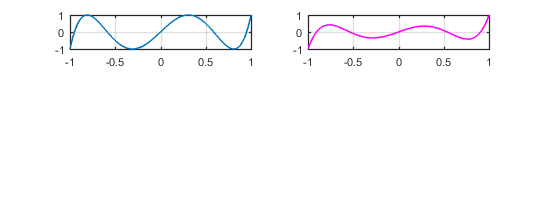
\includegraphics [width=4in]{chap17_05.png}

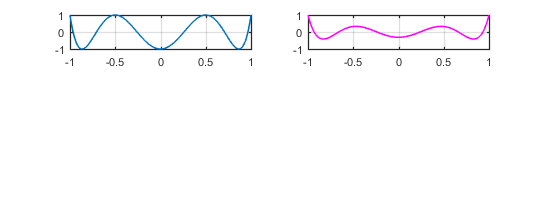
\includegraphics [width=4in]{chap17_06.png}
\begin{par}
 \vskip 1pt 
\end{par} \vspace{1em}
\begin{par}
For Legendre polynomials normalized by $P_j(1)=1$, the orthogonality condition turns out to be
\end{par} \vspace{1em}
\begin{par}
 \vspace{-1em}
$$ \int_{-1}^1 P_j(x) \kern1pt P_k(x) \kern 1pt dx
= \cases{0 & $j\ne k,$ \cr\noalign{\vskip 5pt}
\displaystyle{2\over 2k+1} & $j=k.$}
\eqno (17.5) $$
\vspace{-1.5em} 
\end{par} \vspace{1em}
\begin{par}
We can verify this formula numerically by constructing what Chebfun calls a \textbf{quasimatrix} $X$, that is, a ``matrix'' whose columns are chebfuns, and then taking inner products of each column with each other column via the quasimatrix product $X^T\! X$. One way to construct $X$ is like this:
\end{par} \vspace{1em}
\begin{par}
 \vskip -2em 
\end{par} \vspace{1em}
\begin{verbatim}
X = [P{1} P{2} P{3} P{4} P{5} P{6}];
\end{verbatim}
\begin{par}
Another equivalent method is built into \texttt{legpoly}:
\end{par} \vspace{1em}
\begin{par}
 \vskip -2em 
\end{par} \vspace{1em}
\begin{verbatim}
X = legpoly(1:6);
\end{verbatim}
\begin{par}
Here is the quasimatrix product.
\end{par} \vspace{1em}
\begin{par}
 \vskip -2em 
\end{par} \vspace{1em}
\begin{verbatim}
X'*X
\end{verbatim}

        \color{lightgray} \begin{verbatim}ans =
    0.6667   -0.0000   -0.0000    0.0000    0.0000    0.0000
   -0.0000    0.4000   -0.0000    0.0000   -0.0000    0.0000
   -0.0000   -0.0000    0.2857   -0.0000    0.0000   -0.0000
   -0.0000    0.0000   -0.0000    0.2222   -0.0000    0.0000
    0.0000   -0.0000    0.0000   -0.0000    0.1818   -0.0000
    0.0000    0.0000   -0.0000    0.0000   -0.0000    0.1538
\end{verbatim} \color{black}
    \begin{par}
This matrix of inner products looks diagonal, as it should, and we can confirm the diagonal structure by checking the norm of the off-diagonal terms:
\end{par} \vspace{1em}
\begin{par}
 \vspace{-2em} 
\end{par} \vspace{1em}
\begin{verbatim}
norm(ans-diag(diag(ans)))
\end{verbatim}

        \color{lightgray} \begin{verbatim}ans =
   2.2418e-16
\end{verbatim} \color{black}
    \begin{par}
The entries on the diagonal are the numbers $2/3, 2/5, 2/7, \dots$ prescribed by (17.5).
\end{par} \vspace{1em}
\begin{par}

Legendre polynomials satisfy the 3-term recurrence relation
$$ (k+1) P_{k+1}^{}(x) = (2k+1)\kern .7pt
x \kern .4pt P_k^{}(x) - k P_{k-1}^{}(x), \eqno (17.6) $$
which may be compared with the recurrence relation (3.10)
for Chebyshev polynomials.  In general, orthogonal polynomials defined by
(17.1)--(17.2) always satisfy a 3-term recurrence relation, and the
reason is as follows.  Supposing $\{\kern .4pt p_n\}$ are monic for simplicity, one
can determine $p_{n+1}$ by the Gram--Schmidt orthogonalization procedure,
subtracting off the projections of the monic degree $n+1$ polynomial
$x\kern .2pt p_n$ onto each of the polynomials $p_0,\dots,p_n$, with the
coefficient of the projection onto $p_k$ being given
by the inner product $(x\kern .2pt p_n,p_k)$:
$$ p_{n+1} = x\kern .2pt p_n - (x\kern .2pt p_n,p_n) p_n - (x\kern .2pt p_n,p_{n-1})p_{n-1} -
\cdots - (x\kern .2pt p_n,p_0)p_0. $$
For every $k<n-1$, however, the inner product is equal to $0$ because
$p_n$ is orthogonal to the lower degree polynomial $x\kern .2pt p_k$:\footnote{What
makes this calculation work, abstractly speaking, is that the
operation of multiplication of a function by
$x$ is self-adjoint with respect to the inner product (17.1).
It is for the same reason of self-adjointness
that the Lanczos iteration in numerical linear algebra, which
applies to real symmetric matrices, reduces them to tridiagonal form, whereas
the Arnoldi iteration, which generalizes Lanczos to arbitrary matrices,
achieves only Hessenberg form [Trefethen \& Bau 1997].}
$$ (x\kern .2pt p_n,p_k) = (\kern .7pt p_n,x\kern .2pt p_k) = 0, \quad k<n-1. \eqno (17.7) $$
Thus the series above reduces to the 3-term recurrence
$$ p_{n+1} = x\kern .2pt p_n - (x\kern .2pt p_n,p_n) p_n - (x\kern .2pt p_n,p_{n-1})p_{n-1}. \eqno (17.8) $$
When the weight function $w$ is even, the middle term drops
out (Exercise 17.5), and the formula further simplifies to
$$ p_{n+1} = x\kern .2pt p_n - (x\kern .2pt p_n,p_{n-1})p_{n-1}\quad \hbox{for $w$ even}. \eqno (17.9) $$
We reiterate that (17.8) and (17.9) are based on the
assumption that the polynomials $\{\kern .4pt p_k\}$ are monic.  For
other normalizations, $p_{n+1}$ must be multiplied by a suitable
constant.

\end{par} \vspace{1em}
\begin{par}
Chebyshev polynomials are not orthogonal in the standard inner product:
\end{par} \vspace{1em}
\begin{par}
 \vskip -2em 
\end{par} \vspace{1em}
\begin{verbatim}
X = chebpoly(1:6); X'*X
\end{verbatim}

        \color{lightgray} \begin{verbatim}ans =
    0.6667         0   -0.4000   -0.0000   -0.0952         0
    0.0000    0.9333    0.0000   -0.3619         0   -0.0825
   -0.4000   -0.0000    0.9714         0   -0.3492    0.0000
   -0.0000   -0.3619         0    0.9841   -0.0000   -0.3434
   -0.0952   -0.0000   -0.3492   -0.0000    0.9899   -0.0000
         0   -0.0825   -0.0000   -0.3434         0    0.9930
\end{verbatim} \color{black}
    \begin{par}
Nevertheless, Legendre and Chebyshev polynomials have much in common, as is further suggested by plots of $T_{50}$ and $P_{50}$:
\end{par} \vspace{1em}
\begin{par}
 \vskip -2em 
\end{par} \vspace{1em}
\begin{verbatim}
T50 = chebpoly(50); P50 = legpoly(50);
subplot(2,1,1), plot(T50), axis([-1 1 -2.5 2.5]), FS = 'fontsize';
grid on, title('Chebyshev polynomial T_{50}',FS,9)
subplot(2,1,2), plot(P50,'m'), axis([-1 1 -.3 .3])
grid on, title('Legendre polynomial P_{50}',FS,9)
\end{verbatim}

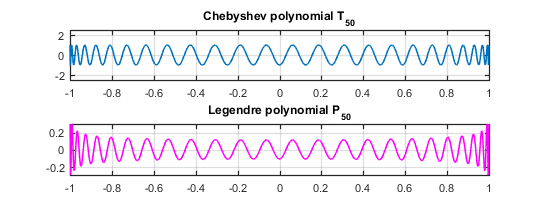
\includegraphics [width=4in]{chap17_07.png}
\begin{par}
 \vskip 1pt 
\end{par} \vspace{1em}
\begin{par}
The zeros of the two families of polynomials are similar, as can be confirmed by comparing Chebyshev (dots) and Legendre (crosses) zeros for degrees 10, 20, and 50.  (Instead of using the \texttt{roots} command here, one could achieve the same effect with \texttt{chebpts(n,1)} and \texttt{legpts(n)}---see Chapter 19.)
\end{par} \vspace{1em}
\begin{par}
 \vskip -2em 
\end{par} \vspace{1em}
\begin{verbatim}
T10 = chebpoly(10); P10 = legpoly(10);
Tr = roots(T10); Pr = roots(P10);
MS = 'markersize'; clf, plot(Tr,.8,'.b',MS,9), hold on
plot(Pr,0.9,'xm',MS,4)
T20 = chebpoly(20); P20 = legpoly(20);
Tr = roots(T20); Pr = roots(P20);
plot(Tr,0.4,'.b',MS,9), plot(Pr,0.5,'xm',MS,4)
Tr = roots(T50); Pr = roots(P50);
plot(Tr,0,'.b',MS,9), plot(Pr,0.1,'xm',MS,4)
axis([-1 1 -.1 1.1]), axis off
\end{verbatim}

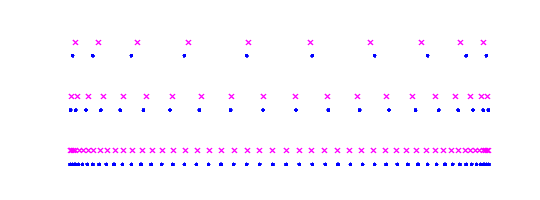
\includegraphics [width=4in]{chap17_08.png}
\begin{par}
 \vskip 1pt 
\end{par} \vspace{1em}
\begin{par}

Asymptotically as $n\to\infty$, both sets of zeros cluster near $\pm 1$
with the same density distribution $n \mu(x)$, with $\mu$ given by (12.10).
This behavior is made precise in Theorem 12.1.4 of
[Szeg\H o 1939] (Exercise 17.7),
and exploitation of more detailed asymptotic properties of Gauss--Jacobi
polynomials is the crucial idea of [Hale \& Townsend 2012].

\end{par} \vspace{1em}
\begin{par}
Another comparison between Chebyshev and Legendre points concerns their Lebesgue functions and Lebesgue constants. Here we repeat a computation of Lebesgue functions from Chapter 15 for 8 Chebyshev points and compare it with the analogous computation for 8 Legendre points. Chebyshev and Legendre points as we have defined them so far differ not just in which polynomials they are connected with, but in that Chebyshev points come from extrema whereas Legendre points come from zeros.
\end{par} \vspace{1em}
\begin{par}
 \vskip -2em 
\end{par} \vspace{1em}
\begin{verbatim}
hold off
s = chebpts(8); [L,Lconst] = lebesgue(s);
subplot(1,2,1), plot(L), grid on, hold on, plot(s,L(s),'.'), Lconst
ylim([0,5]), title('Chebyshev points, n=7',FS,9)
s = legpts(8); [L,Lconst] = lebesgue(s);
subplot(1,2,2), plot(L), grid on, hold on, plot(s,L(s),'.'), Lconst
ylim([0,5]), title('Legendre points, n=7',FS,9)
\end{verbatim}

        \color{lightgray} \begin{verbatim}Lconst =
    2.2022
Lconst =
    4.5135
\end{verbatim} \color{black}
    
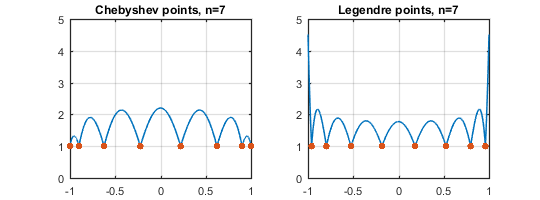
\includegraphics [width=4in]{chap17_09.png}
\begin{par}
 \vskip 1pt 
\end{par} \vspace{1em}
\begin{par}
The Lebesgue functions and constants for Legendre points are a little bigger than for Chebyshev points, having size $O(n^{1/2})$ rather than $O(\log n)$ because of behavior near the endpoints $\hbox{[Szeg\H o 1939, p.\ 338]}$.  This small difference is of little significance for most applications: the Lebesgue constants are still quite small, and either set of points will usually deliver excellent interpolants.
\end{par} \vspace{1em}
\begin{par}
Moreover, an alternative is to consider \textit{Legendre extreme points}---the $n+1$ points in $[-1,1]$ at which $|P_n(x)|$ attains a local maximum. (The Legendre extreme points in $(-1,1)$ are also the roots of the Jacobi polynomial $P^{(1,1)}(x)$.) The Lebesgue function in this case looks even more satisfactory:
\end{par} \vspace{1em}
\begin{par}
 \vskip -2em 
\end{par} \vspace{1em}
\begin{verbatim}
clf
s = [-1; roots(diff(legpoly(7))); 1]; [L,Lconst] = lebesgue(s);
subplot(1,2,1), plot(L), grid on, hold on, plot(s,L(s),'.'), Lconst
ylim([0,5]), title('Legendre extreme points, n=7',FS,9)
s15 = [-1; roots(diff(legpoly(15))); 1]; [L,Lconst] = lebesgue(s15);
subplot(1,2,2), plot(L), grid on, hold on, plot(s15,L(s15),'.'), Lconst
ylim([0,5]), title('Legendre extreme points, n=15',FS,9)
\end{verbatim}

        \color{lightgray} \begin{verbatim}Lconst =
    1.9724
Lconst =
    2.4303
\end{verbatim} \color{black}
    
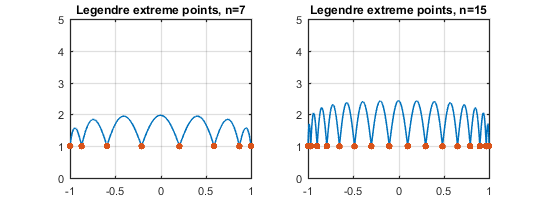
\includegraphics [width=4in]{chap17_10.png}
\begin{par}
 \vskip 1pt 
\end{par} \vspace{1em}
\begin{par}
The Legendre extreme points have a memorable property: as shown by Stieltjes [1885], they are the Fekete or minimal-energy points in $[-1,1]$, solving the equipotential problem on that interval for a finite number of equal charges (Exercise 12.1). Here, for example, is a repetition of a figure from Chapter 11 but now for 8 Legendre extreme points instead of 8 Chebyshev points. Again the behavior is excellent.
\end{par} \vspace{1em}
\begin{par}
 \vspace{-2em} 
\end{par} \vspace{1em}
\begin{verbatim}
ell = poly(s,domain(-1,1));
clf, plot(s,ell(s),'.k',MS,10)
hold on, ylim([-0.9,0.9]), axis equal
xgrid = -1.5:.02:1.5; ygrid = -0.9:.02:0.9;
[xx,yy] = meshgrid(xgrid,ygrid); zz = xx+1i*yy;
ellzz = ell(zz); levels = 2.^(-6:0);
contour(xx,yy,abs(ellzz),levels,'k')
title(['Curves |l(x)| = 2^{-6}, 2^{-5}, ..., 1 '...
    'for 8 Legendre extreme points'],FS,9)
\end{verbatim}

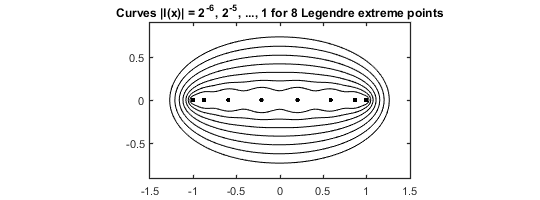
\includegraphics [width=4in]{chap17_11.png}
\begin{par}

\vspace{1em}
\begin{displaymath}
\framebox[4.7in][c]{\parbox{4.5in}{\vspace{2pt}\sl
{\sc Summary of Chapter 17.}
Chebyshev polynomials are just one example of a family of polynomials
orthogonal with respect to a weight function $w(x)$ on $[-1,1]$. For
$w(x) = \hbox{constant}$,
one gets the Legendre polynomials.\vspace{2pt}}}
\end{displaymath}

\end{par} \vspace{1em}
\begin{par}
 \smallskip\small\parskip=2pt
\par
{\bf Exercise 17.1.  Chebyshev and Legendre Lebesgue constants.}
Extend the experiments of the text to a table and a plot of Lebesgue
constants of Chebyshev, Legendre, and Legendre extreme points for
interpolation in $n+1$ points with $n = 1,2,4,\dots, 256$.  (To compute
Legendre extreme points efficiently, you can use the observation about
Jacobi polynomials mentioned in the text and the Chebfun command \verb|jacpoly|.)
What asymptotic behavior do you observe as $n\to\infty$?
\par
{\bf Exercise 17.2.  Chebyshev and Legendre interpolation points.}
Define $f(x) = x\tanh(2\sin(20x))$, and let $p$ and $p_L^{}$ be the
interpolants to $f$ in $n+1$ Chebyshev or Legendre points on $[-1,1]$, respectively.
The latter can be computed with \verb|interp1| as in Chapter~13.
(a) For $n+1 = 30$, plot $f$, $p$, and $p_L^{}$.  What are the $\infty$-norm
errors $\|f-p\|$ and $\|f-p_L^{}\|$?
(b) For $n+1 = 300$, plot $f-p$ and $f-p_L^{}$.  What are the errors now?
\par
{\bf Exercise 17.3.  Orthogonal polynomials via QR decomposition.}
(a) Construct a Chebfun quasimatrix {\tt A} with columns corresponding to
$1,x,\dots,x^5$ on $[-1,1]$.  Execute {\tt [Q,R] = qr(A)} to find an
equivalent set of orthonormal functions, the columns of {\tt Q}, and plot
these with {\tt plot(Q)}. How do the columns of {\tt Q} compare with the
Legendre polynomials
normalized by (17.3)?  (b) Write a {\bf for} loop to normalize
the columns of {\tt Q} in a fashion corresponding to
$P_j(1) = 1$ and to adjust $R$ correspondingly so that the
product {\tt Q*R} continues to be equal to {\tt A}, up to rounding
errors, and plot the new quasimatrix with {\tt plot(Q)}.
How do the columns of the new {\tt Q} compare with the
Legendre polynomials normalized by $P_j(1)=1$?
\par
{\bf Exercise 17.4.  Zeros of orthogonal polynomials.}  Let
$\{\kern .4pt p_n\}$ be a family of orthogonal polynomials on $[-1,1]$ defined
by (17.1)--(17.2).  Show by using (17.2) that the zeros of $p_n$
are distinct and lie in $(-1,1)$.
\par
{\bf Exercise 17.5.  Even and odd orthogonal polynomials.} Suppose the
weight function $w$ of (17.1) is even.  Prove by induction that $p_n$ is
even when $n$ is even and odd when $n$ is odd.
\par
{\bf Exercise 17.6.  Legendre and Chebyshev differential equations.}
(a) Show from the recurrence relation (17.6) that
the Legendre polynomial $P_n$ satisfies the differential
equation $(1-x^2) P'' - 2x P' + n(n+1)P = 0$.
(b) Show from (3.10) that
the Chebyshev polynomial $T_n$ satisfies the differential
equation $(1-x^2) T'' - x T' + n^2T = 0$.
[This exercise needs more.]
\par
{\bf Exercise 17.7.  The envelope of an orthogonal polynomial.}
Theorem 12.1.4 of [Szeg\H o 1939] asserts that as $n\to\infty$, the
envelope of an orthonormal polynomial $p_n$ defined by (17.1)--(17.3)
approaches the curve $(w_{\tiny\hbox{CHEB}}^{}(x)/w(x))^{1/2}$, where
$w_{\tiny\hbox{CHEB}}^{}$ is the Chebyshev weight (17.4).
Explore this prediction numerically with plots of Legendre polynomials
for various $n$.
\par
{\bf Exercise 17.8.  Minimality of orthogonal polynomials.}
Let $\{\kern .4pt p_n\}$ be the family of monic orthogonal polynomials associated
with the inner product (17.1).  Show that if $q$ is any monic polynomial
of degree $n$, then $(q,q) \ge (\kern .7pt p_n,p_n)$.
\par 
\end{par} \vspace{1em}



\end{document}
    
